% Another 2-cochain g on the Klein bottle, with values on the blue edges.
% Source: book/tex/homology/cohomology.tex (§ Visualization of cohomology groups).
\documentclass[border=2mm]{standalone}
\usepackage{tikz}
\usepackage{amssymb}
\usetikzlibrary{arrows.meta,decorations.markings}
\tikzset{midarrow/.style={postaction={decorate},decoration={
  markings,mark=at position 0.55 with {\arrow{Latex[length=2mm]}}}}}
\begin{document}
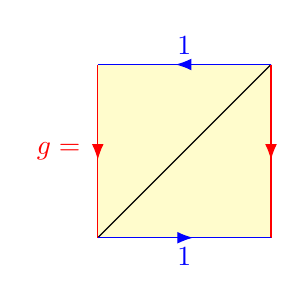
\begin{tikzpicture}[scale=2.2]
  \fill[yellow!20] (0,0) rectangle (1,1);
  \draw (1,1) -- (0,0);
  \draw[red, midarrow]  (1,1) -- (1,0);
  \draw[blue, midarrow] (0,0) -- (1,0) node[midway, below] {$1$};
  \draw[red, midarrow]  (0,1) -- (0,0) node[midway, left] {$g = {}$};
  \draw[blue, midarrow] (1,1) -- (0,1) node[midway, above] {$1$};
\end{tikzpicture}
\end{document}
